\section{Metodologia}\label{sec:metodologia}

Esta seção apresenta a instanciação do método utilizada nos experimentos. Conforme discutido na Seção \ref{sec:kernel_pipeline}, as escolhas descritas a seguir (modelo, amostra, fontes, \textit{kernels} e transformações) não fazem parte do método e foram realizadas para demonstrar o seu funcionamento. Qualquer pipeline núcleo-transformação produz uma matriz semidefinida positiva e, consequentemente, uma pseudométrica, mas nada na forma do método garante que a geometria resultante diga algo sobre o modelo que a originou. A pergunta que orienta esta seção é, portanto: ``a geometria induzida reflete o comportamento do modelo?''.

Validar a geometria não significa mostrar que o espaço separa classes, visto que um espaço construído sobre as ativações de uma rede treinada separa classes quase por construção. A afirmação testada é que as distâncias do espaço preveem o que o modelo faz, isto é, qual classe ele decide, em quais amostras ele erra e quais categorias ele confunde. Por esse motivo, sempre que possível, a referência é algo que o próprio modelo produziu (a predição, o erro e a confusão), e não o rótulo do conjunto de dados. Além disso, as leituras são repetidas sobre onze conjuntos de dados, várias sementes e três arquiteturas, cada afirmação é reportada como a fração das execuções em que ela se sustenta e toda leitura é acompanhada de uma referência de nulidade, ou piso (Subseção \ref{subsec:pisos}).

\subsection{Perguntas que orientam os experimentos}\label{subsec:perguntas}

A pergunta central se desdobra em oito perguntas, que determinam os experimentos e a ordem em que os resultados são apresentados na Seção \ref{sec:resultados}. Cada uma é respondida contra uma referência externa à geometria, visto que uma pergunta cuja resposta dependa apenas da própria geometria não pode ser respondida pelo método que a produziu.

\begin{enumerate}
    \item[\textbf{P1.}] \textit{A geometria reflete o comportamento do modelo?} As distâncias preveem qual classe o modelo decide, em quais amostras ele erra e quais classes ele confunde? A referência é o comportamento do próprio modelo, e o piso é a mesma construção sobre o modelo não treinado.

    \item[\textbf{P2.}] \textit{A composição acrescenta algo às fontes isoladas?} Se a matriz de Gram conjunta não superar a fonte de ativações, o produto de Hadamard seria apenas uma forma mais custosa de ler as ativações.

    \item[\textbf{P3.}] \textit{O método se distingue de uma simples CKA?} A matriz de Gram do método é centrada e normalizada, o mesmo tipo de objeto sobre o qual a CKA opera. A pergunta não é respondida pelo valor do alinhamento, e sim pelo conteúdo: a parte da Gram que a CKA não enxerga carrega informação sobre o comportamento do modelo?

    \item[\textbf{P4.}] \textit{A energia espectral descreve como o modelo representa cada amostra?} O subespaço retido $V_r$ contém as direções que separam as decisões do modelo, e a energia que escapa dele, medida por $\widehat{E}_{\mathrm{ratio}}$, sinaliza as amostras em que o modelo erra?

    \item[\textbf{P5.}] \textit{Tomando as posições de uma imagem como objetos, o campo de energia e os conjuntos de nível apontam o que o modelo utiliza na entrada?} A pergunta tem três partes, reportadas separadamente: se a energia se concentra sobre o objeto (verificado pela máscara de segmentação), se as regiões de maior energia sustentam a decisão (verificado por deleção) e se os conjuntos de nível reúnem as regiões que o modelo representa de forma semelhante.

    \item[\textbf{P6.}] \textit{Por que esta amostra foi classificada de forma diferente daquela?} Essa é a forma local e contrastiva do método. A amostra comparada é um contrafactual da amostra explicada, no sentido da Seção \ref{sec:referencial}, e a resposta é um ranking de atributos ou de regiões. A validação é feita por intervenção sobre a entrada: levar os primeiros atributos do ranking ao valor do contrafactual deve mudar a decisão do modelo.

    \item[\textbf{P7.}] \textit{As leituras dependem do modelo?} As fontes da Subseção \ref{subsec:fontes} não fazem referência à convolução, e o mesmo código é aplicado a um perceptron multicamadas, a uma rede convolucional e a um transformador. Na sua forma mais forte, a pergunta é se o método é de fato modelo-agnóstico, e ela é respondida aplicando-o a uma árvore de decisão.

    \item[\textbf{P8.}] \textit{Em que profundidade a decisão se forma?} As leituras por bloco produzem uma datação da decisão, que é comparada a uma datação independente, obtida por intervenção $do(\cdot)$ sobre os estados internos.
\end{enumerate}

P1 é a pergunta da qual as demais dependem: se a geometria não refletir o comportamento do modelo, as demais leituras descreveriam um espaço sem relação com ele. As perguntas P1 a P4 tomam cada amostra como um objeto, P5 aplica-se apenas às imagens, P6 e P8 são respondidas com intervenções, sobre a entrada e sobre os estados internos, e P7 repete as leituras sobre outros modelos.

\subsection{Bases de dados}\label{subsec:dados}

O primeiro conjunto de bases reúne dez bases tabulares do OpenML \citep{Vanschoren2014}, descritas na Tabela \ref{tab:bases}, sete das quais integram o OpenML-CC18 \citep{Bischl2021}. Os critérios de seleção foram fixados antes das medições: todas são multiclasse (de 3 a 26 classes), possuem ao menos duas mil amostras e não possuem classes com pouquíssimos exemplos. A \texttt{covertype} é subamostrada de forma estratificada para 30\,000 amostras. Os atributos são padronizados pelas estatísticas do treino, e a partição é estratificada em 70\% para treino, 10\% para validação e 20\% para teste.

\begin{table}[htbp]
\centering
\caption{Bases tabulares utilizadas, com o identificador no OpenML, o número de amostras (após a subamostragem, no caso da \texttt{covertype}), de atributos e de classes, e a referência de origem. A última coluna indica as bases que integram o OpenML-CC18 \citep{Bischl2021}.}
\label{tab:bases}
\footnotesize
\setlength{\tabcolsep}{4pt}
\begin{tabular}{l r r r r l c}
\hline
Base & OpenML & Amostras & Atributos & Classes & Origem & CC18 \\
\hline
\texttt{letter} & 6 & 20\,000 & 16 & 26 & \citet{FreySlate1991} & sim \\
\texttt{pendigits} & 32 & 10\,992 & 16 & 10 & \citet{UCIPendigits} & sim \\
\texttt{optdigits} & 28 & 5\,620 & 64 & 10 & \citet{AlpaydinKaynak1998} & sim \\
\texttt{satimage} & 182 & 6\,430 & 36 & 6 & \citet{UCISatimage} & sim \\
\texttt{segment} & 36 & 2\,310 & 19 & 7 & \citet{UCISegment} & não \\
\texttt{har} & 1478 & 10\,299 & 561 & 6 & \citet{Anguita2013} & sim \\
\texttt{mfeat-factors} & 12 & 2\,000 & 216 & 10 & \citet{vanBreukelen1998} & sim \\
\texttt{gas-drift} & 1476 & 13\,910 & 128 & 6 & \citet{Vergara2012} & não \\
\texttt{dna} & 40670 & 3\,186 & 180 & 3 & \citet{Michie1994} & sim \\
\texttt{covertype} & 1596 & 30\,000 & 54 & 7 & \citet{Blackard1999} & não \\
\hline
\end{tabular}
\end{table}

O segundo conjunto é o Oxford-IIIT Pet \citep{Parkhi2012}, com 7\,349 fotografias de 37 raças de gatos e cachorros, a partição oficial em 3\,680 imagens de \textit{trainval} e 3\,669 de teste e uma máscara de segmentação por imagem. As imagens são recortadas no centro em $128\times128$ píxeis, e a máscara recebe o mesmo recorte. A máscara nunca entra no treinamento nem na construção das matrizes de Gram: ela é a verdade externa contra a qual as leituras espaciais são verificadas. A base impõe um regime de dados escassos, com cerca de noventa imagens de treino por raça.

Todas as bases têm mais de duas classes, e isso é deliberado. Em uma tarefa binária, a margem contrastiva definida adiante se reduz à diferença entre dois logits, e trocar a predição inverte o sinal do gradiente em toda a rede, de modo que qualquer \textit{kernel} sensível a sinal separa as duas populações por construção. As matrizes de Gram por objeto são construídas sobre um subconjunto balanceado do teste, com $n \approx 500$ objetos sorteados com semente fixa e sem aumento de dados.

\subsection{Modelos e treinamento}\label{subsec:modelo}

São utilizadas três arquiteturas com a mesma estrutura de sondagem: sete estados, denotados por \texttt{stem} e \texttt{b1} a \texttt{b6}, em que o ponto de sondagem é sempre a saída do bloco. Nas bases tabulares, o modelo é um perceptron multicamadas residual com seis blocos de largura 256, da forma $h_{\ell} = \mathrm{ReLU}\bigl(\mathrm{BN}(W_2\,\mathrm{ReLU}(\mathrm{BN}(W_1 h_{\ell-1}))) + h_{\ell-1}\bigr)$, seguidos de uma cabeça linear. Nas imagens, o primeiro modelo é uma ResNet \citep{He2016} de três estágios, com dois blocos residuais cada e larguras de 64, 128 e 256 canais. O segundo é um transformador de visão com tokenizador convolucional \citep{Hassani2021}, em que o estado de cada bloco é mantido na forma espacial $(C, H, W)$ e as projeções do bloco são convoluções $1\times1$, idênticas a camadas lineares por \textit{token}. Assim, as mesmas fontes são extraídas das duas redes de imagem sem nenhuma alteração do código.

Todos os modelos são treinados do zero, com os hiperparâmetros da Tabela \ref{tab:hiperparametros}, cinco sementes por base tabular e três sementes por arquitetura nas imagens. Essa escolha não é acessória: o piso das leituras de comportamento é o mesmo modelo com os pesos da inicialização, gravados antes da primeira época, e uma inicialização pré-treinada já carregaria geometria aprendida. No Oxford-IIIT Pet, a ResNet atinge acurácia de teste de $0{,}672 \pm 0{,}010$ e o transformador, $0{,}439 \pm 0{,}005$. A diferença é esperada para um transformador treinado do zero com poucos dados, e as comparações do método são sempre relativas ao piso do próprio modelo.

\begin{table}[htbp]
\centering
\caption{Hiperparâmetros de treinamento. O aumento de dados é aplicado apenas ao conjunto de treino, e a amostra utilizada nas matrizes de Gram e em todas as leituras não é aumentada.}
\label{tab:hiperparametros}
\small
\setlength{\tabcolsep}{4pt}
\begin{tabular}{>{\raggedright\arraybackslash}p{0.19\linewidth} >{\raggedright\arraybackslash}p{0.36\linewidth} >{\raggedright\arraybackslash}p{0.36\linewidth}}
\hline
 & Bases tabulares (MLP residual) & Oxford-IIIT Pet (ResNet e transformador) \\
\hline
Otimizador & Adam & SGD com momento de Nesterov $0{,}9$ (ResNet) e AdamW (transformador) \\
Taxa de aprendizado & $10^{-3}$ & \textit{one-cycle}, máxima $0{,}05$ (ResNet) e $10^{-3}$ (transformador) \\
Decaimento de pesos & $10^{-4}$ & $5\times10^{-4}$ (ResNet) e $0{,}05$ (transformador) \\
Épocas & até 100, com parada antecipada (paciência 15) & 120 \\
Tamanho do lote & 256 & 64 \\
Função de perda & entropia cruzada, suavização $0{,}05$ & entropia cruzada, suavização $0{,}05$ (ResNet) e $0{,}1$ (transformador) \\
Aumento de dados & nenhum & espelhamento horizontal, recorte aleatório, variação de cor e apagamento aleatório \\
Mistura de amostras & nenhuma & \textit{mixup} ou \textit{cutmix} em metade dos lotes \\
Sementes & 0 a 4 & 0 a 2 \\
\hline
\end{tabular}
\end{table}

\subsection{As três fontes indexadas por objeto}\label{subsec:fontes}

Cada objeto $z_i$ é representado, no domínio produto da Definição \ref{def:tensor_sim}, por $d = 3$ fontes extraídas do mesmo bloco, que descrevem o estado do bloco, a sensibilidade da decisão a esse estado e os parâmetros que produzem esse estado.

A primeira fonte são as ativações ($A$), isto é, o estado de saída do bloco, reduzido por \textit{pooling} médio a uma grade comum de $4\times4$ posições e achatado como $A_i \in \mathbb{R}^{C \times P}$, com $P = 16$ nas imagens e $P = 1$ nos modelos tabulares.

A segunda fonte é o gradiente contrastivo ($\Gamma$), a derivada, com respeito ao mesmo estado, da margem entre o logit de uma classe de referência e a média dos logits das demais,
\begin{equation}\label{eq:margem}
    m(z_i) = f_{c^\star}(z_i) - \frac{1}{K-1}\sum_{c \neq c^\star} f_c(z_i).
\end{equation}
Tomar $c^\star$ como a classe predita torna circulares as leituras referidas à predição, visto que o gradiente passa a carregar a própria predição. No perceptron, por exemplo, a classe predita explica 100\% da variação de $\Gamma$ em \texttt{b6}. Por esse motivo, as leituras referidas ao comportamento utilizam um \textbf{alvo fixo}, isto é, a mesma classe de referência para todos os objetos. Representações sem geometria, como $\Gamma$ no último bloco sob alvo fixo, são marcadas como indefinidas.

A terceira fonte são os parâmetros ativados ($W$), isto é, os filtros que o objeto de fato ativou. Sendo $W \in \mathbb{R}^{C \times F}$ os pesos da camada de saída do bloco e $u_i$ o vetor de ativação média por canal,
\begin{equation}\label{eq:fonte_parametros}
    p_i[:,s] \;=\; \sum_{c=1}^{C} A_i[c,s]\, W[c,:] \;\in\; \mathbb{R}^{F},
    \qquad
    \langle p_i, p_j\rangle \;=\; u_i^\top (WW^\top) u_j .
\end{equation}
A matriz de Gram dos filtros é a mesma para todos os objetos e, portanto, não pode indexá-los. Na construção \eqref{eq:fonte_parametros}, ela reaparece como a forma bilinear da fonte, ponderada pela ativação de cada objeto.

\subsection{Construção das matrizes de Gram}\label{subsec:construcao}

Para cada bloco e cada fonte $l \in \{W, A, \Gamma\}$, a matriz de Gram bruta é calculada com \textit{kernel} linear, recebe a transformação angular $T_a$ da Tabela \ref{tab:T_catalog} e é deslocada para o intervalo $[0,1]$. As três componentes são compostas pelo produto de Hadamard do Corolário \ref{cor:hadamard_form}, e o resultado é centrado e normalizado em traço:
\begin{equation}\label{eq:componente}
    \mathbf{G}_l \;=\; \frac{T_a(\widetilde{\mathbf{G}}_l) + \mathbf{J}}{2},
    \qquad
    \mathbf{G} \;=\; T_{\mathrm{tr}}\Bigl(T_c\bigl(\mathbf{G}_W \circ \mathbf{G}_A \circ
    \mathbf{G}_\Gamma\bigr)\Bigr),
\end{equation}
em que $\mathbf{J} = \mathbf{1}\mathbf{1}^\top$. A partir de $\mathbf{G}$ é obtida a pseudodistância $d_{\mathbf{G}}^2(i,j) = G_{ii} + G_{jj} - 2G_{ij}$ da Equação \eqref{eq:gram_distance}. A Figura \ref{fig:gram_construcao} ilustra cada etapa.

Cada escolha responde a um problema concreto. O \textit{kernel} linear preserva a interação multiplicativa entre as fontes, enquanto, com \textit{kernels} gaussianos, o produto de Hadamard se reduz identicamente a uma soma das métricas das fontes. A normalização angular impede que a fonte de maior amplitude domine a composição: sem ela, a ordenação do produto concorda com a do gradiente entre $0{,}95$ e $1{,}00$. O deslocamento por $\mathbf{J}$, que é semidefinida positiva, evita que o produto de três cossenos em torno de zero torne a Gram conjunta numericamente diagonal, e o centramento remove a direção uniforme que esse deslocamento injeta no espectro.

\begin{figure}[htbp]
\centering
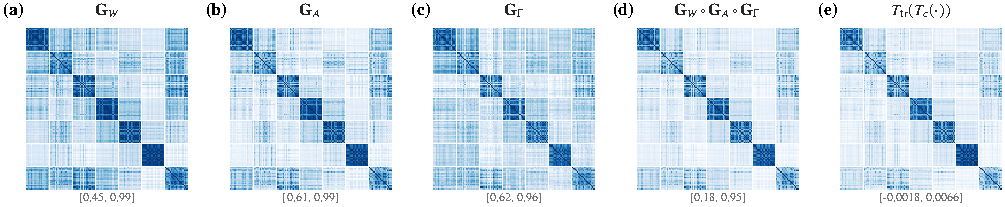
\includegraphics[width=\textwidth]{figuras/gram_construcao.pdf}
\caption{Construção da matriz de Gram, ilustrada sobre a base \texttt{segment} (sete classes, vinte amostras por classe), no bloco \texttt{b3} do perceptron multicamadas com alvo fixo. Da esquerda para a direita são apresentadas as matrizes de Gram componentes ($\mathbf{G}_W$, $\mathbf{G}_A$ e $\mathbf{G}_\Gamma$), o produto de Hadamard que as compõe e a matriz de Gram após o centramento e a normalização em traço. Os objetos estão ordenados por classe, com as fronteiras entre as classes marcadas por linhas claras, e tons escuros indicam maior similaridade.}
\label{fig:gram_construcao}
\end{figure}

\subsection{Experimentos}\label{subsec:experimentos}

Os experimentos são divididos em cinco famílias, de acordo com a referência que cada uma utiliza, além da datação por intervenção.

A \textbf{primeira família} (P1 e P2) reúne as leituras da matriz de distância: a acurácia de $k$-vizinhos \textit{leave-one-out} contra a predição do modelo, a área sob a curva ROC da margem geométrica como preditora do acerto e a correlação de Spearman, no nível de classe, entre a proximidade geométrica dos pares de classes e a \textbf{confusão suave}, isto é, a probabilidade média que o modelo atribui à classe $b$ nas amostras da classe $a$, simetrizada e calculada sobre o teste inteiro.

A \textbf{segunda família} (P4) reúne as leituras do espectro, obtidas da decomposição $\mathbf{G} = V\Lambda V^\top$: a fração das direções de classe contida em $V_r$ e a razão de energia ortogonal $\widehat{E}_{\mathrm{ratio}}$ como preditora do erro. Como essas leituras dependem de $r$, as comparações entre representações utilizam o mesmo $r = K-1$ para todas, para que uma diferença no número de modos retidos não seja lida como uma diferença de geometria.

A \textbf{terceira família} (P2 e P3) reúne as ablações e referências: cada fonte isolada, a análise representacional clássica (RSA) com distância euclidiana sobre as ativações e a decomposição contra a CKA, $\hat{\mathbf{G}} = a\,\hat{K}_{\mathrm{ativ}} + R$, com $a = \mathrm{CKA}(\mathbf{G}, K_{\mathrm{ativ}})$. Cada parte é projetada no cone semidefinido positivo, registrando-se a massa espectral descartada, e avaliada pelas leituras de comportamento.

A \textbf{quarta família} (P5) toma como objetos as posições espaciais de uma única imagem e reúne o campo de energia e os conjuntos de nível, validados pela máscara do animal e por deleção, conforme detalhado na Subseção \ref{subsec:res_campo}.

A \textbf{quinta família} (P6) é a leitura contrastiva e contrafactual do método. Para cada amostra $i$ classificada corretamente, toma-se como par a amostra $j$ mais próxima de $i$ nos atributos entre aquelas que o modelo classifica de outra forma. Pela definição da Seção \ref{sec:referencial}, $j$ é um contrafactual observado de $i$, o vizinho mais próximo de classe distinta \citep{KeaneSmyth2020}. A pergunta é quais das diferenças entre $i$ e $j$ importam para o modelo. Nos dados tabulares, cada atributo $f$ recebe a pontuação
\begin{equation}\label{eq:delta_d}
    \Delta d_f \;=\; d(i,j) - d(i^{(f)},j),
\end{equation}
em que $i^{(f)}$ é a amostra $i$ com o atributo $f$ levado ao valor de $j$, e $d$ é a distância da Gram conjunta com alvo fixo. Isto é, $\Delta d_f$ mede quanto a intervenção $do(x_f := x_{j,f})$ aproxima $i$ do seu contrafactual no espaço do modelo. Essa leitura exige apenas as $F + 2$ linhas formadas por $i$, $j$ e as $F$ versões de $i$ com um atributo trocado. A validação é externa à geometria e constrói contrafactuais sintéticos: trocam-se os $k$ primeiros atributos do ranking e mede-se se a predição de $i$ passa a ser a de $j$, como faz o algoritmo NICE \citep{Brughmans2024}. Um ranking melhor produz um contrafactual válido com menos trocas, isto é, mais próximo de $i$. Nas imagens, a unidade é a região, as posições das duas imagens entram em uma única matriz de Gram de ordem $2P$ e a validação é a deleção das regiões na ordem do mapa, medindo a margem $f_{c_i} - f_{c_j}$.

Por fim, a \textbf{datação} (P8) é obtida por intervenção sobre os estados internos. Em modo de inferência, a rede é um modelo causal estrutural determinístico e sem confundimento, em que $h_\ell = f_\ell(h_{\ell-1})$, de modo que a intervenção pode ser executada diretamente, em vez de estimada \citep{Pearl2009}:
\begin{equation}\label{eq:intervencao}
    R(\ell,\sigma) \;=\; \Pr\Bigl(\hat{y} \neq \hat{y}_{\text{limpo}}
    \;\Bigm|\; do\bigl(h_\ell := h_\ell + \sigma\,s_\ell \odot \varepsilon\bigr)\Bigr),
    \qquad \varepsilon \sim \mathcal{N}(0, I),
\end{equation}
em que $s_\ell$ é o vetor de desvios-padrão por canal do bloco, o que torna $\sigma$ um orçamento comparável entre blocos.

\subsection{Estudos de caso}\label{subsec:estudos_caso}

As famílias anteriores medem se as leituras se sustentam entre bases e sementes, mas comparam o método apenas com pisos e referências simples. Dois estudos de caso sobre a base \texttt{letter} \citep{FreySlate1991} complementam essa avaliação. A base foi escolhida porque os seus dezesseis atributos têm significado (posição e dimensões da caixa que envolve a letra, número de píxeis acesos, momentos e contagens de bordas), porque possui 26 classes e porque, com $F = 16$, o valor de Shapley de um par pode ser calculado de forma exata. Até onde sabemos, a base não havia sido objeto de um estudo de interpretabilidade.

\subsubsection*{O método, o SHAP, o LIME e uma árvore de decisão sobre o mesmo modelo}

O primeiro estudo responde a P6 e compara o método às duas técnicas de atribuição mais utilizadas, o SHAP \citep{LundbergLee2017} e o LIME \citep{Ribeiro2016}, ambas modelo-agnósticas. O modelo explicado é o perceptron multicamadas, com cinco sementes e cem pares contrafactuais por semente, escolhidos como na quinta família. O ranking do método é o da Gram conjunta de \texttt{b3}.

Cada técnica é avaliada em duas formas. A \textbf{forma contrastiva} explica a margem $m = f_{c_j} - f_{c_i}$ tomando $j$ como referência, e responde à mesma pergunta que o método. No SHAP, ela inclui o valor de Shapley exato do jogo $v(S) = m(x_j^{S}, x_i^{\bar S}) - m(x_i)$, isto é, o \textit{baseline Shapley} com $j$ de referência \citep{SundararajanNajmi2020}, e o SHAP intervencional usual lido como $\phi_m(x_j) - \phi_m(x_i)$. No LIME, o modelo linear local é ajustado sobre $m$ em torno de $x_i$, e cada atributo é pontuado pela variação prevista ao levá-lo ao valor de $j$. A \textbf{forma usual} explica apenas a amostra $i$, como as técnicas costumam ser aplicadas. O valor de Shapley exato é a decomposição da própria troca que o teste contrafactual mede e, por isso, funciona como o limite superior do teste. Como o método não amostra e tem custo fixo por par, as técnicas também são comparadas com o mesmo orçamento de avaliações do modelo, estimando o Shapley por permutações amostradas \citep{Strumbelj2014} e variando o número de perturbações do LIME.

A árvore de decisão \citep{Breiman1984} é treinada diretamente sobre os rótulos, sem acesso ao perceptron. Para um par $(i,j)$, a explicação da própria árvore é o atributo do nó em que os caminhos de $i$ e de $j$ se separam, e a leitura é a posição desse atributo em cada ranking, nos pares em que a árvore reproduz as duas predições do perceptron. A árvore é uma corroboração, e não uma verdade de referência: a concordância indica que dois modelos independentes se apoiam nos mesmos atributos. No nível global, as importâncias do método, do SHAP, do LIME e da árvore são comparadas com a importância por permutação no perceptron \citep{Breiman2001}.

\subsubsection*{O método aplicado a uma árvore de decisão}

O segundo estudo responde a P7 na sua forma mais forte. Se o método é modelo-agnóstico, aplicá-lo a um modelo sem ativações contínuas nem gradiente deve exigir apenas outra escolha de fontes. Além disso, a árvore explica a si mesma pelo seu caminho de decisão, o que fornece uma resposta conhecida.

Nesta instanciação, os blocos são as profundidades $\ell$ da árvore, e cada amostra possui três fontes em cada profundidade. A fonte de \textbf{caminho} é o indicador dos nós visitados até $\ell$, o estado da árvore. A fonte de \textbf{folga} registra, em cada nó já atravessado, a quantidade $(x_f - t)/\sigma_f$, isto é, quanto falta para a amostra mudar de ramo. A fonte de \textbf{classes} é a distribuição de classes do nó atual, o que a árvore decidiria naquele ponto. A composição e a leitura de pares são as mesmas das redes.

A árvore fornece três referências. A primeira é o atributo do nó de separação, que deve ser o primeiro do ranking. A segunda é a profundidade dessa separação, que deve coincidir com a profundidade em que esse atributo passa a ser o primeiro do método, verificando a datação de P8 contra uma resposta exata. A terceira é o contrafactual mínimo, isto é, o menor conjunto de trocas que muda a predição da árvore, obtido por enumeração dos $2^{16}$ subconjuntos. O piso é o método aplicado a uma árvore treinada sobre rótulos embaralhados.

\subsection{Referências de nulidade}\label{subsec:pisos}

Um piso indica o valor de uma leitura se a geometria não carregasse nenhuma informação, e apenas a geometria deve mudar entre a medida e o seu piso. Nas leituras referidas ao comportamento, medir o modelo não treinado contra a sua própria predição mudaria a geometria e o alvo ao mesmo tempo, e além disso é degenerado: na inicialização, a predição se concentra em uma única classe na maior parte da amostra, o que a torna trivial de recuperar. Por esse motivo é adotado o \textbf{piso cruzado}, em que a geometria do modelo não treinado é medida contra o comportamento do modelo treinado, de modo que a única diferença entre a medida e o piso é o treinamento.

Três pisos adicionais acompanham leituras específicas. Nas leituras espaciais, um mapa que marca apenas o centro da imagem, visto que o animal tende a ocupar o centro. Nas leituras de pares, um piso de especificidade, o mesmo mapa calculado contra uma terceira amostra de classe não envolvida, visto que um mapa que não o supera indica o que importa em $i$, e não o que distingue $i$ de $j$. Nas leituras de pares, também a ordem aleatória entre os atributos que diferem. Por fim, as comparações entre representações são estritas, de modo que empates não contam como vitória, e leituras indefinidas são excluídas da contagem, e não tratadas como falhas.

\subsection{Reprodutibilidade}\label{subsec:reprodutibilidade}

Todos os experimentos utilizam semente fixa na partição dos dados, na seleção da amostra, na inicialização e nas intervenções estocásticas. Cada execução grava um relatório com todas as medidas, os seus pisos e a configuração completa, de modo que qualquer tabela pode ser reconstruída sem repetir o treinamento. O método está disponível como a biblioteca \texttt{fannar}, que implementa o pipeline núcleo-transformação para matrizes de Gram arbitrárias, as leituras e as fontes das duas instanciações. Quanto ao custo, a análise do método está na Subseção \ref{subsec:custo}. A instanciação acrescenta a extração das fontes, uma passagem direta e uma reversa por objeto, isto é, $\Theta(nT)$ para um modelo cuja passagem direta custa $T$ \citep{GriewankWalther2008}, e a leitura de um par custa $\Theta\bigl(F\,T\bigr)$, contra $\Theta\bigl(2^F\,T\bigr)$ do valor de Shapley exato. O treinamento de cada modelo leva de poucos minutos a cerca de uma hora em uma única placa gráfica.
